\chapter{Fault-Tolerance Design and Behavioral Framework\label{cha:chapter6}}

This chapter theoretically formalizes the mathematical foundations, distributed behavior patterns, and cyber-physical recovery protocols of our masterless multi-robot system, which are critical to its resilience. Whereas the steady-state behavior of the system under study is formalized in Chapter 5, industrial environments pose a significant challenge to robust and deterministic task finishing. Specifically, Section 6.1 describes the general fault classification and asynchronous dual-channel detection mechanism, whereas Sections 6.2--6.3 detail the hierarchical process of localization-dependent state recovery and progress-based kinematic stall detection. Section 6.4 then describes the reactive parallel-axis goal shifting paradigm used for obstacle avoidance, followed by a description of the decentralized blacklist propagation mechanism and associated state granularities in Section 6.5. Finally, Section 6.6 formulates the battery-aware decentralized task re-allocation protocol, while Section 6.7 outlines the analytical redundancy and exception-based failure switching mechanisms for the vision pipeline. Taken together, all components comprise the system-level fault resilience framework synthesized in Section 6.8.

\section{Fault Taxonomy and Asynchronous Dual-Channel Detection}

The decentralized multi-robot system under study incurs both computational and physical faults during its execution, which require careful taxonomical classification as system-specific state transitions. Particularly, the presence of large-scale multi-robot logistics platforms in confined spaces makes the distinction between physical and computational anomalies challenging due to the close interrelation of the robots' spatial and task allocation states.

\subsection{Formal Classification of Fault Modes}

Consistent with the fleet's edge-processing architecture, our multi-robot system makes the non-Byzantine assumption, namely, that faulty robots do not publish any deceptive or altered messages over the communication network. Instead, the system focuses on detecting and responding to silent (fail-silent) and stopping (fail-stop) anomalies ~\cite{okumura2023fault}. Consider the spatial state of the $i$-th robot, $\mathbf{x}_i(t) = [x_i(t), y_i(t), \psi_i(t)]^T \in \text{SE}(2)$.

A fail-silent manifestation corresponds to an abrupt failure of a robot's perception, decision-making, and communication components, depriving the other robots of the information about the failed robot's state, as formalized in Equation~\eqref{eq:fail_silent_state}:
\begin{equation} \lim_{\tau \to 0^+} \mathbf{x}_i(t + \tau) = \emptyset \label{eq:fail_silent_state} \end{equation}
In practice, such a failure could be triggered by a sudden power loss or hardware malfunction that renders the robot's computer or communication module inoperational.

Unlike the fail-silent mode, a robot entering a fail-stop state powers down its drive trains but continues to execute the edge perception and communication algorithms. Such a category of faults incorporates non-destructive physical collisions and localization upsets, after which the robot is still capable of performing diagnostic and localization checks.

Formally, these failure modes are described within our decentralized state machine via the following transition conditions:
\begin{enumerate}
    \item \textbf{Resource exhaustion fault and subsequent failsafe shutdown:} The robot's battery level $E_i(t)$ reaches the lowest possible charge $E_{\text{fail}} = 0.0\%$. To maximize the audit throughput of active units and avoid narrow-aisle deadlock hazards associated with low-power return-to-dock maneuvers, the robot continues to track its trajectory until its battery is completely depleted before transitioning to the \texttt{FAILED} state. Subsequently, the robot deallocates all occupied spatial resources (e.g., trajectory segments) and allows the other robots to take over its residual tasks~\cite{bolu2021adaptive}.
    \item \textbf{Localization uncertainty increase beyond the safety threshold:} $\sigma_{\text{amcl}} \ge \sigma_{\text{threshold}}$, suspending path tracking to prevent collisions.
    \item \textbf{Kinematic stall:} Motion being hindered by unmodeled obstacle or a local minimum in the navigation function, with the robot's commanded velocity \texttt{cmd\_vel} not corresponding to the actual robot velocity.
\end{enumerate}

The non-Byzantine nature of the detected faults is the result of deliberate design choices driven by the physical constraints of the problem at hand. Particularly, large-scale logistics operations typically take place within confined areas with no access to external networks. It is therefore unviable to utilize computationally heavy Byzantine-specific cryptography, consensus reaching algorithms, or digital signature verification procedures on resource-constrained embedded processors ~\cite{strobel2020blockchain, roth2021byzantine}.

\subsection{Asynchronous Dual-Channel Model: Self-Declaration vs. Passive Heartbeats}

The proposed model enables the fleet to tolerate failures with reduced overhead by implementing both explicit self-declarations and passive, peer-to-peer heartbeats as failure detection channels. Contrary to the perfect loopback channel assumption in simulated settings, wireless communication is bound to exhibit packet loss in an industrial environment. To this end, the fleet employs an explicit declaration channel to handle soft fail-stops (e.g., depleted battery or kinematic stall). Such conditions prompt the affected agent to kill its drive processes, abort active navigation, and publish a JSON object with \texttt{FAILED} status and its coordinates to the status topic for the peer discovery.

In addition, the fleet utilizes a passive heartbeat-timeout channel to detect both soft and hard fail-silence conditions. Every active agent $a_j \in \mathcal{A}$ should periodically publish a heartbeat message with a predefined frequency $f_{\text{hb}} = 1.0\,\text{Hz}$. Assuming $t_{\text{last}, j}$ denotes the timestamp of the last received message from $a_j$, any observer agent $a_i \in \mathcal{A} \setminus \{a_j\}$ can tentatively mark $a_j$ as failed at each time $t_i$ if the following condition is satisfied:
\begin{equation} t - t_{\text{last}, j} > T_{\text{timeout}} \label{eq:heartbeat_timeout_formula} \end{equation}
where $T_{\text{timeout}} = 5.0\,\text{s}$.

The choice of $T_{\text{timeout}} = 5.0\,\text{s}$ at $f_{\text{hb}} = 1.0\,\text{Hz}$ renders the timeout long enough to mitigate packet losses while still keeping the false-positive rate acceptable. As a practical matter, steel warehouses are prone to develop multipath fading and shadowing due to their infrastructure ~\cite{zadeh2025fast}, thus calling for reliable communication models. In particular, packet losses can be modeled as independent Bernoulli trials with probability $p_{\text{loss}} \in [0.0, \; 1.0]$. Let us define $n = T_{\text{timeout}} \cdot f_{\text{hb}} = 5$ as the number of consecutive missed heartbeats required to declare $a_j$ failed. Then, the probability of falsely re-allocating a failed agent's tasks equals:
\begin{equation} \mathbb{P}(\text{False Alarm}) = p_{\text{loss}}^n = p_{\text{loss}}^5 \label{eq:bernoulli_false_alarm} \end{equation}
At $p_{\text{loss}} = 0.20$ (a reasonable estimate given the harsh radio conditions), a simple calculation yields:
\begin{equation} \mathbb{P}(\text{False Alarm}) = 0.20^5 = 0.00032 \quad (0.032\%) \label{eq:false_alarm_calculation} \end{equation}
which renders the false-positive probability negligibly small. On the other hand, reducing the timeout to $T_{\text{timeout}} = 2.0\,\text{s}$ ($n=2$) would cause the false alarm probability to jump to $0.20^2 = 0.04$ ($4.0\%$). Thus, such a setting would cause frequent, disruptive task reallocations due to spurious failure declarations. At the same time, increasing $T_{\text{timeout}}$ to $15.0\,\text{s}$ would lead to excessive delays in failure detection, thereby prolonging the time to recovery and adding to the overall makespan. Therefore, $T_{\text{timeout}} = 5.0\,\text{s}$ offers a reasonable trade-off between minimizing both false-positive rates and detection latency.The state transitions of both explicit self-declaration and passive heartbeat-timeout detection channels leading to dynamic task re-allocation are summarized in Figure~\ref{fig:dual_channel_detection}.

\begin{figure}[htbp]
\centering
\includegraphics[width=0.6\textwidth]{fig_6_1_dual_channel_detection.pdf}
\caption{State diagram of the asynchronous dual-channel fault detection mechanism detailing explicit self-declarations for soft fail-stops and passive heartbeat timeouts for hard fail-silent states.}
\label{fig:dual_channel_detection}
\end{figure}

\subsection{Scalability Limits and \texorpdfstring{$O(N^2)$}{O(N^2)} Overhead of Distributed Subscriptions}

While the described failure detection mechanism eliminates the single point of failure associated with the dispatch server, it incurs a significant $\mathcal{O}(N^2)$ overhead in terms of both computation and communication. In particular, every active agent should subscribe to all peer topics in order to monitor their statuses, incurring substantial overhead on the vehicle's CPU and the shared Wi-Fi link.

Let us denote the number of robots in the fleet by $N$. Then, the number of required subscriptions scales as $\mathcal{O}(N^2)$ because every agent should subscribe to all peer topics in $\mathcal{A} \setminus \{a_i\}$. Given the frequency $f_{\text{hb}}$ and the size of individual packets $S_{\text{packet}}$, the resulting bandwidth consumption equals:
\begin{equation} R_{\text{traffic}} = N(N - 1) \cdot f_{\text{hb}} \cdot S_{\text{packet}} \label{eq:network_traffic_scale} \end{equation}
which could become substantial under heavy network loads. In particular, such a setting may emerge when a large number of robots $N$ reside in the warehouse. In this case, the bandwidth consumption will quickly overwhelm the shared Wi-Fi access point, thereby increasing $p_{\text{loss}}$ (the packet loss probability) in the process. Consequently, the false-positive rate will follow Eq.~\ref{eq:false_alarm_calculation}, limiting the practical value of larger fleets. Hence, $f_{\text{hb}} = 1.0\,\text{Hz}$ emerges as a reasonable choice that prevents the shared access point from becoming a new single point of failure.

\subsection{Idempotency Under Redundant Reallocation Triggers}

Given the asynchronous nature of the publication-subscription model, it is possible that multiple agents observe a failed heartbeat at different times and attempt to reallocate tasks concurrently. This situation gives rise to several potential inconsistencies, including redundant inspection point allocations and contention over shared resources. To address this issue, the task reallocation operator should be designed to be idempotent, i.e., applying it multiple times should yield the same result as applying it once. We formalize this notion as follows.

Let us denote by $\mathcal{M} = [\mathcal{M}_{i,k}]_{i,k}$ the configuration matrix that encodes the current assignment of inspection points $p_k \in \mathcal{P}$ to robots $a_i \in \mathcal{A}$. In particular, $\mathcal{M}_{i,k} = 1$ if and only if inspection point $p_k$ is allocated to robot $a_i$. Given the failure detection mechanism from Section 6.1, each surviving agent $a_i$ is aware of a subset of failed peers $\Phi_i(t) \subset \mathcal{A}$. At any time $t$, the reallocation operator $\mathcal{R}$ defines the updated configuration matrix as:
\begin{equation} \mathcal{R}: \mathcal{M} \to \mathcal{M}' \label{eq:reallocation_operator_definition} \end{equation}
Whenever agent $a_i$ observes a failed heartbeat from agent $a_{\text{failed}}$, it updates its configuration matrix $\mathcal{M}_i$ according to Eq.~\ref{eq:reallocation_operator_definition}. To this end, agent $a_i$ maintains a set of failed peers $\Phi_i(t)$ and checks if $a_{\text{failed}}$ is in $\Phi_i(t)$:\footnote{At the software implementation level, this logical set $\Phi_i(t)$ is decoupled into two separate memory registers: \texttt{health\_\allowbreak monitor.\allowbreak failed\_\allowbreak robots} (used to trigger local calculations) and \texttt{processed\_\allowbreak failed\_\allowbreak robots} (used to filter incoming \texttt{/add\_waypoints} ROS~2 broadcasts).}
\begin{equation} a_{\text{failed}} \in \Phi_i(t) \label{eq:processed_set_check} \end{equation}
If this condition is satisfied, the observed heartbeat message has already been taken into account and no further action is necessary. Conversely, if $a_{\text{failed}} \notin \Phi_i(t)$, agent $a_i$ adds $a_{\text{failed}}$ to its tracking state via:
\begin{equation} \Phi_i(t^+) = \Phi_i(t) \cup \{ a_{\text{failed}} \} \label{eq:processed_set_update} \end{equation}
and updates its configuration matrix $\mathcal{M}_i$ in accordance with Eq.~\ref{eq:reallocation_operator_definition}. This way, each agent utilizes the information about failed peers to reserve new inspection points for itself. As a result, the idempotency condition:
\begin{equation} \mathcal{R} \left( \mathcal{R} \left( \mathcal{M} \right) \right) = \mathcal{R}\left( \mathcal{M} \right) \label{eq:idempotency_proof} \end{equation}
holds true for any two agents $a_i$ and $a_j$. In particular, it becomes possible to prevent redundant allocation attempts by maintaining a consistent view of failed peers. The same mechanism can be used to handle a sequence of consecutive failures, as described in more detail in Section 6.6.3. Specifically, the revised allocation matrix $\mathcal{M}'$ is computed afresh every time a new failure is detected, taking into account the remaining workload. This approach is sufficient to preserve consistency within the fleet's configuration.

\section{Hierarchical State Recovery and Localization Stability}\label{sec:ch6_hierarchical_recovery}

Robust mobile navigation in unconstrained warehouse environments requires maintaining accurate spatial state estimates of the robot's position on the global map. Sudden accelerations, wheel slippage on slippery concrete, and extended traversal of structurally similar shelving units may lead to imprecise localization updates, causing the global filter to drift away from the true robot pose~\cite{fox2003kld}. The two-stage hierarchical recovery procedure detailed below is used to recover from such events.

\subsection{Covariance-Triggered Fault Identification \& The Cyber-Physical Costmap Margin Paradox}\label{sec:ch6_margin_paradox}

The localization fault identification procedure begins once the robot's covariance estimates report a decrease in the accuracy of the global pose tracking by the localization filter. The pose covariance matrix is monitored as $\mathbf{\Sigma}_p$ in Equation~\eqref{eq:amcl_covariance_matrix}:
\begin{equation} \mathbf{\Sigma}_p = \begin{bmatrix} \sigma_{xx}^2 & \sigma_{xy}^2 & \sigma_{x\psi}^2 \\ \sigma_{yx}^2 & \sigma_{yy}^2 & \sigma_{y\psi}^2 \\ \sigma_{\psi x}^2 & \sigma_{\psi y}^2 & \sigma_{\psi\psi}^2 \end{bmatrix} \in \mathbb{R}^{3 \times 3} \label{eq:amcl_covariance_matrix} \end{equation}
with diagonal entries representing the variance in meters of the position state in the map reference frame. The \texttt{amcl\_pose} covariance is subsequently used by the recovery module to formulate an isotropic measure of the localization uncertainty:
\begin{equation} \sigma_{\text{amcl}} = \sqrt{\sigma_{xx}^2 + \sigma_{yy}^2} \label{eq:sigma_amcl_derivation} \end{equation}
against an acceptable baseline value:
\begin{equation} \sigma_{\text{amcl}} \le \sigma_{\text{baseline}} \label{eq:strict_uncertainty_threshold} \end{equation}
during which $\sigma_{\text{baseline}} = 0.15\,\text{m}$. At this level of uncertainty, the mobile robot would be incapable of safely navigating narrow passageways due to the possibility of collision with physical obstacles.

Meanwhile, during the initial spool up of the localization filter and large scale maneuvers around the warehouse perimeter, wheel slip can cause intermittent surges in the covariance value. A premature initiation of the recovery procedure due to $\sigma_{\text{amcl}} > \sigma_{\text{baseline}} = 0.15\,\text{m}$ would lead to unnecessary interruptions in the overall floor throughput by recovery-specific procedures, which is why a relaxed operational threshold is also introduced to the localization gate:
\begin{equation} \sigma_{\text{threshold}} = \sigma_{\text{relax}} = 0.50\,\text{m} \label{eq:relaxed_uncertainty_threshold} \end{equation}
with the robot's operational envelope defined by the narrowest aisle width $W_{\text{aisle}} = 2.25\,\text{m}$. Given the robot's overall diameter of $D_{\text{robot}} = 0.54\,\text{m}$ ($0.27\,\text{m}$ bounding radius), the corresponding side clearance at the center of the aisle is:
\begin{equation}
\begin{aligned}
M_{\text{physical}} &= \frac{W_{\text{aisle}} - D_{\text{robot}}}{2} \\
&= \frac{2.25 - 0.54}{2} = 0.855\,\text{m}
\end{aligned}
\label{eq:physical_clearance_margin}
\end{equation}
but using the physical margin $M_{\text{physical}}$ as a collision avoidance margin involves the cyber-physical costmap inflation paradox. Namely, while local path planners in ROS typically utilize a set of layered costmaps~\cite{lu2014layered}, the obstacle layer in particular utilizes a global inflation radius of $r_{\text{global\_inflation}} = 0.55\,\text{m}$ which decreases the allowable margin before a \texttt{local\_map} obstacle layer to:
\begin{equation} M_{\text{inflation}} = M_{\text{physical}} - r_{\text{global\_inflation}} = 0.855 - 0.55 = 0.305\,\text{m} \label{eq:cyber_physical_margin} \end{equation}
By approximating the robot's lateral position tracking error $e_y$ as a zero mean Gaussian with variance $\sigma^2_{\text{amcl}}$, the cumulative probability of a robot side sweeping the local planner's lethal obstacle buffer can be estimated with the standard normal Q-function. In practice, the one-dimensional approximation for the standard deviation $\sigma_{\text{amcl}}$ used for this calculation is selected conservatively as:
\begin{equation} \mathbb{P}(\text{Inflation Breach}) = 2 Q\left( \frac{M_{\text{inflation}}}{\sigma_{\text{amcl}}} \right) \label{eq:collision_probability_q_function} \end{equation}
The comparison between the value under two different localization gates illustrates the trade-off between the conservative single-frame position estimates and the ability to operate within narrow workspaces:

Under the baseline localization gate $\sigma_{\text{amcl}} = \sigma_{\text{baseline}} = 0.15\,\text{m}$, the Q-value evaluates to:
\begin{equation} \mathbb{P}(\text{Inflation Breach}) = 2 Q\left( \frac{0.305}{0.15} \right) = 2 Q(2.03) \approx 0.0424 \quad (4.24\%) \label{eq:collision_prob_baseline} \end{equation}
which presents an acceptable physical margin for driving on the centerline of a narrow aisle.

Meanwhile, under the higher $\sigma_{\text{amcl}} = \sigma_{\text{relax}} = 0.50\,\text{m}$, the probability density corresponds to:
\begin{equation} \mathbb{P}(\text{Inflation Breach}) = 2 Q\left( \frac{0.305}{0.50} \right) = 2 Q(0.61) \approx 0.5418 \quad (54.18\%) \label{eq:collision_prob_relax} \end{equation}
presenting a $54\%$ chance of crossing into the local planner's lethal obstacle layer mid-operation.

Using this localization gate as a trigger for the two-stage recovery procedure provides sufficient time to pause active path following to avoid collisions while still allowing the robot to perform necessary recovery operations in open staging areas.

\subsection{Stage 1: Local Spin Recovery and Bounded Dwell Constraints}

With the localization estimate crossing the $\sigma_{\text{amcl}} > \sigma_{\text{threshold}}$ gate, the robot interrupts its active path follower and initiates Stage 1: Local Spin Recovery in order to reset the particle filter distribution. This is achieved by centering the robot's movement program on a rotation in place in order to allow rangefinders to observe nearby structural landmarks~\cite{karakaya2026cg}.

First, the robot zeroes out its translational velocity component $v_x = 0.0\,\text{m/s}$ while initiating a slow angular rotation sweep:
\begin{equation} \omega_z = 0.3\,\text{rad/s} \label{eq:spin_velocity_command} \end{equation}
the magnitude of which is limited to $0.3\,\text{rad/s}$ in order to allow the laser scanners to acquire a high-quality 360-degree spatial sample without motion-induced blur.

At the same time, in order to avoid premature convergence on a single observation during the rotation, the spin rate is also limited by a minimum dwell time requirement:
\begin{equation} t_{\text{spin}} \ge T_{\text{dwell}} \label{eq:dwell_time_constraint} \end{equation}
with $T_{\text{dwell}} = 8.0\,\text{s}$ defining the minimum time spent at a fixed angle during the rotation. With a $0.3\,\text{rad/s}$ spin rate, this corresponds to a 137-degree rotation, allowing the laser scanners to track a sufficient number of different structural landmarks (building walls, rack faces) to allow the particle filter to converge to a consistent estimate.

The robot is only allowed to resume normal operations when the pose uncertainty falls below the threshold for three consecutive frames:
\begin{equation} \sigma_{\text{amcl}}(t_{k - m}) < \sigma_{\text{threshold}} \quad \forall m \in \{0, 1, 2\} \label{eq:stable_exit_condition} \end{equation}
in order to avoid resuming localization following a single, isolated observation. This allows the robot to avoid localization resets due to individual spurious observations while resuming normal operations only once stable tracking is re-established.

\subsection{Stage 2: Global Reinitialization, State Escalation, and Lease Persistence Mechanics}

If the robot is unable to satisfy the $\sigma_{\text{amcl}} < \sigma_{\text{threshold}}$ condition within $T_{\text{stage1}} = 22.0\,\text{s}$ of entering Stage 1, the robot proceeds to Stage 2: Global Reinitialization in order to resume normal operations. In particular, the active localization filter is globally reinitialized in order to avoid getting stuck in a permanent divergence state.

The process of reinitialization consists in spreading out the particle filter state across the available workspace $\mathcal{W}_{\text{free}}$, thus removing the robot's current position estimate from consideration. In order to allow the particle filter to converge to a consistent estimate, the robot undergoes another rotation procedure analogous to Eq.~\ref{eq:spin_velocity_command}. However, due to the computational cost of global reinitialization and the resulting position uncertainty, the Stage 2 recovery procedure has its own recovery budget:
\begin{equation} n_{\text{recovery}} \le N_{\text{max}} \label{eq:recovery_attempts_limit} \end{equation}
with $N_{\text{max}} = 2$ in order to avoid excessive resource expenditure on localization recovery.

If the robot is still unable to pass the $\sigma_{\text{amcl}} < \sigma_{\text{threshold}}$ test after exhausting the global recovery budget, it results in the current goal becoming unrecoverable. As a result, the robot releases its only spatial claim and returns the target to the unassigned queue for subsequent claim processing by other robots. The robot then resumes its decision-making cycle in order to select a new target for processing without requiring a system-wide alert.

Meanwhile, during the long spin-down periods of Stages 1 and 2, the robot must carefully renew its spatial corridor leases in order to avoid deadlocks in narrow aisles. In particular, when a robot is engaged in a prolonged rotation procedure inside a narrow aisle, the lease for the corridor section it occupies may expire before it finishes the rotation. As a result, a different robot entering the same aisle from the opposite direction will be able to successfully claim the same section, and will proceed to perform its own rotation procedure at the center of the aisle. Once the first robot finishes its localization recovery procedure, it will find itself unable to exit the aisle due to the second robot occupying the only available section, forcing both robots to simultaneously retry their recovery procedures.

In order to avoid this deadlock scenario, the lease renewal procedure is separated from the robot's ability to move through the environment. In particular, the claim renewal procedure runs as an independent thread at a fixed $T_{\text{renew}} = 1.5\,\text{s}$ interval regardless of the robot's current state. As a result, as long as the robot is not formally \texttt{FAILED}, its current location lease:
\begin{equation} t_{\text{expire}} = t + \tau_{\text{lease}} \label{eq:lease_calculation} \end{equation}
with $\tau_{\text{lease}} = 6.0\,\text{s}$ is renewed at every cycle, keeping its exclusive access to the corridor section open until it completes the spin recovery procedure. This ensures that a robot performing a prolonged recovery spin is able to retain its access to the aisle, keeping its egress path available once it finishes the procedure.The overall execution flow of the two-stage recovery procedure, along with the independent spatial lease-renewal thread, is illustrated in Figure~\ref{fig:hierarchical_recovery}.

\begin{figure}[htbp]
\centering
\includegraphics[width=0.85\textwidth]{fig_6_2_hierarchical_recovery.pdf}
\caption{Flowchart of the two-stage hierarchical localization recovery mechanism, highlighting the transition from Stage~1 local spin recovery to Stage~2 global reinitialization and the independent corridor lease persistence thread.}
\label{fig:hierarchical_recovery}
\end{figure}

\begin{figure}[htbp]
\centering
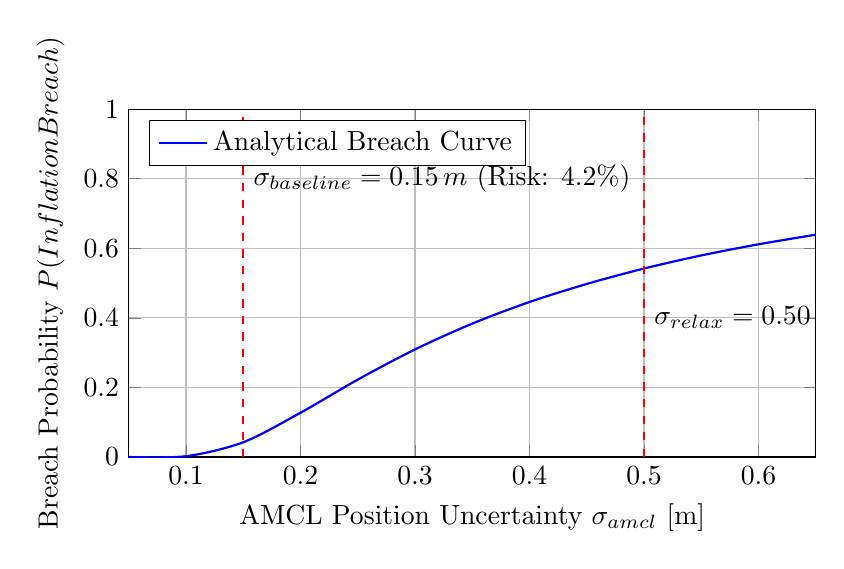
\begin{tikzpicture}
\begin{axis}[
    xlabel={AMCL Position Uncertainty $\sigma_{\text{amcl}}$ [m]},
    ylabel={Breach Probability $\mathbb{P}(\text{Inflation Breach})$},
    xmin=0.05, xmax=0.65,
    ymin=0, ymax=1.0,
    grid=both,
    minor grid style={dashed, gray!30},
    major grid style={gray!50},
    width=0.85\textwidth,
    height=6cm,
    legend pos=north west
]
\addplot[thick, blue, smooth] coordinates {
    (0.05, 0.0000)
    (0.10, 0.0023)
    (0.15, 0.0424)
    (0.20, 0.1272)
    (0.25, 0.2224)
    (0.30, 0.3092)
    (0.35, 0.3834)
    (0.40, 0.4456)
    (0.45, 0.4974)
    (0.50, 0.5418)
    (0.55, 0.5794)
    (0.60, 0.6114)
    (0.65, 0.6390)
};
\addlegendentry{Analytical Breach Curve}

\draw[red, dashed, thick] (axis cs:0.15,0) -- (axis cs:0.15,1.0) 
    node[pos=0.8, right, black] {$\sigma_{\text{baseline}} = 0.15\,\text{m}$ (Risk: 4.2\%)};
    
\draw[red, dashed, thick] (axis cs:0.50,0) -- (axis cs:0.50,1.0)
    node[pos=0.4, right, black] {$\sigma_{\text{relax}} = 0.50\,\text{m}$ (Risk: 54.2\%)};
\end{axis}
\end{tikzpicture}
\caption{Cyber-physical costmap inflation breach probability $\mathbb{P}(\text{Inflation Breach})$ as a function of the localization uncertainty metric $\sigma_{\text{amcl}}$ under a cyber-physical safety margin of $M_{\text{inflation}} = 0.305\,\text{m}$.}
\label{fig:cyber_physical_margin_plot}
\end{figure}

\section{Progress-Based Kinematic Stall Detection and Physical Escape}

Robots moving their bodies inside a logistics warehouse may encounter temporary work\-space confinements. While the global planner computes paths based on fixed facility layout, the local trajectory controller must avoid dynamically extruded obstacle boundaries. To physically bypass such planning constraints and restore the agent's free mobility, we implement the progress-based kinematic stall detection and localization-aware escape policy.

\subsection{Time-Integrated Position Progress Filter versus Motor Current Estimation}

The majority of collision and stall detectors in the mobile logistics domain rely on robot drive motor current estimation to infer the presence of unexpected physical interactions with the environment ~\cite{xiang2025servo}. The current estimation module operates on the assumption that any external mechanical resistance raises the drive motor torque beyond the expected value, manifesting as an anomalous current draw in the corresponding drive motor. However, most logistics facilities have a concrete floor with friction significantly lower than that expected in the average home environment. As such, the robot's differential wheels experience an abrupt loss of grip when physically entrapped by an unmapped obstacle or a local planning minimum.

At the moment of such robot-obstacle engagement, the robot's differential wheels spin freely due to the smoothness of the floor. As a result, the torque and, consequently, the drive motor current remain near their steady-state operating values. Hence, the current-based collision estimation module fails to detect the stall because its perception of external mechanical resistance does not account for the robot's differential locomotion. Instead, we propose using the position progress time-integrated filter that tracks the robot's spatial progress relative to the global map frame.

Let $\mathbf{p}(t) = [x(t), y(t)]^T \in \mathbb{R}^2$ denote the filtered position coordinates of the robot footprint in the global map frame at a given moment $t$. The time-integrated spatial progress over a moving time window $T_{\text{window}}$ is defined as:
\begin{equation}
\thinmuskip=1mu\medmuskip=1mu\thickmuskip=2mu
d_{\text{progress}}(t) = \|\mathbf{p}(t) - \mathbf{p}(t - T_{\text{window}})\|_2 = \sqrt{\left(x(t) - x(t - T_{\text{window}})\right)^2 + \left(y(t) - y(t - T_{\text{window}})\right)^2} \label{eq:spatial_progress_formula}
\end{equation}
With that, the progress-based kinematic stall detector compares the filtered progress value to a configurable progress epsilon to decide whether to initiate the emergency escape procedure:
\begin{equation} d_{\text{progress}}(t) < \delta_{\text{progress}} \label{eq:stall_trigger_condition} \end{equation}
Where the progress epsilon $\delta_{\text{progress}} = 0.03\,\text{m}$ represents the minimum distance the robot should traverse within the timeframe $T_{\text{window}}$ before raising the stall flag.

The emergency escape procedure runs synchronously within the robot's 10 Hz state-machine tick, which binds its internal timer to the current robot goal state. While the configuration retains the dual-timeout setup ($12.0\,\text{s}$ versus $10.0\,\text{s}$) for backward compatibility with the legacy Manhattan routing paradigm, the active local planner utilizes the ablation optimization that bypasses the candidate routing procedure. As such, the watchdog thread binds the emergency escape procedure to the $T_{\text{window, direct}} = 10.0\,\text{s}$ timeout instead to avoid false positives when approaching standard waypoints. If the robot's spatial progress remains below the $\delta_{\text{progress}} = 0.03\,\text{m}$ threshold throughout the designated timeframe, the local planner cancels the active goal and initiates the open-loop physical escape sequence detailed in the following subsection.

\subsection{Progress Epsilon and Localization Noise Floor Cross-Correlation}

The choice of the progress epsilon $\delta_{\text{progress}} = 0.03\,\text{m}$ as a stall detection threshold involves balancing the robot's localization accuracy when stationary against the need to prevent false positives at the beginning of a movement command. Whenever the robot is stationary scanning the shelves or awaiting a higher-level manager instruction, its spatial estimate undergoes rapid centimeter-level oscillations due to the particle filter update procedure.

To mitigate the possibility of localization noise-induced false stalls, one chooses the progress epsilon $\delta_{\text{progress}} = 0.03\,\text{m}$ as a fraction of the localization noise floor, satisfying the following progress filter safety condition:
\begin{equation} \delta_{\text{progress}} = \frac{1}{5} \sigma_{\text{baseline}} = \frac{0.15\,\text{m}}{5} = 0.03\,\text{m} \label{eq:epsilon_noise_separation} \end{equation}
This formulation keeps the time-integrated spatial progress safe from sudden jumps due to localization inaccuracies.

\subsection{Alternating Open-Loop Escapes and Actuator Decoupling}

With the emergency escape procedure invoked, the local planner begins executing the multi-step open-loop escape sequence that temporarily disassociates robot actuation from the costmap obstacle layer for a limited period. The open-loop escape sequence consists of two stages: linear backup and rotational separation.

First, the robot enters the linear backup mode, in which the local planner decouples the chassis from the local costmap and applies a steady negative linear velocity:
\begin{equation} v_x = -0.12\,\text{m/s} \label{eq:escape_linear_velocity} \end{equation}
to move the robot backwards, away from the obstacle. While the linear backup duration is set to a static parameter $t_{\text{config}} = 0.80\,\text{s}$ by the configuration file, the production code utilizes the hardcoded $t_{\text{backup}} = 1.67\,\text{s}$ due to the need to create sufficient clearance. With that, the distance covered during the linear backup phase is equal to:
\begin{equation} d_{\text{backup}} = \lvert v_x \rvert \cdot t_{\text{backup}} = 0.12 \cdot 1.67 = 0.2004\,\text{m} \label{eq:exact_retreat_distance} \end{equation}
Which satisfies the requirement to create enough clearance to remove the robot from the local obstacle layer. However, the linear escape maneuver alone is insufficient to remove the robot from the influence area of the obstacle.

Second, with the robot moved backwards, the local planner initiates the rotational escape procedure that begins right after the linear backup finished. The robot rotates in place to create enough clearance for its front bumper:
\begin{equation} \omega_z = \gamma \cdot 0.35\,\text{rad/s} \label{eq:escape_rotational_velocity} \end{equation}
for a duration of $t_{\text{rotation}} = 0.90\,\text{s}$.

To prevent the robot from oscillating between the two positions when stuck, we apply the following alternating rotation multiplier:
\begin{equation} \gamma = (-1)^{k+1} \label{eq:alternating_direction_multiplier} \end{equation}
which allows the robot to turn left $\gamma = +1$ on the first iteration and then right $\gamma = -1$ on the subsequent attempts. The loop runs a maximum of $N_{\text{escape\_max}} = 5$ times in total before the task is deferred back to the global pool, allowing a peer agent to claim the target. We suggest utilizing the described open-loop physical escape sequence because it safely moves the robot away from the obstacle while minimizing the risk of secondary collisions~\cite{tang2025path}. Figure~\ref{fig:stall_escape_workflow} details the decision pipeline for time-integrated position progress filtering, open-loop linear retreats, and direction-alternating rotational escapes. The complete state machine executing this open-loop physical escape sequence and managing the progress-based stall watchdog is compiled in Appendix~\ref{app:code_recovery} (Listing~\ref{lst:recovery_manager_core}).

\begin{figure}[htbp]
\centering
\includegraphics[width=\textwidth]{fig_6_3_stall_escape_workflow.pdf}
\caption{Progress-based kinematic stall detection and open-loop escape control loop, illustrating the alternating left/right rotational escape strategy and task deferral fallback.}
\label{fig:stall_escape_workflow}
\end{figure}

\section{Reactive Parallel-Axis Coordinate Shifting under Spatial Occlusion}\label{sec:ch6_pythagorean_shift}

In a masterless multi-robot inspection paradigm, the vehicles must be able to navigate their environment while avoiding other robots. A failed agent presents a serious navigational challenge to the rest of the fleet, as collisions with a parked or crashed robot are detrimental to the mission progress. Whenever the robot encounters a condition that prevents it from continuing the inspection task (e.g., localization failure), the agent updates its status to \texttt{FAILED} and physically stops. As such, the failed robot becomes an obstacle whose presence may impede the progress of its peers.

\subsection{Spatial Occlusion Boundary Conditions and Mapping of Failed Peers}

Let us define the position of a failed robot $a_j$ by its coordinates $[px_j, py_j]^T \in \mathbb{R}^2$. Furthermore, assuming that the robot has a physical footprint of a circle of radius $D_{\text{safe}}$, the failed robot presents a circular occlusion region of radius $D_{\text{safe}}$ to the rest of the fleet:
\begin{equation}
\begin{aligned}
\mathcal{B}_j &= \left\{ \mathbf{x} \in \mathbb{R}^2 \mid
\|\mathbf{x} - \mathbf{p}_j\|_2 < D_{\text{safe}} \right\}
\end{aligned}
\label{eq:occlusion_bubble_definition}
\end{equation}
with $D_{\text{safe}} = 0.85\,\text{m}$. Any active inspection target with a nominal target position $\mathbf{q}_{\text{target}} = [x_{\text{target}}, y_{\text{target}}]^T \\ \in \mathbb{R}^2$ located within the circular region:
\begin{equation} \mathbf{q}_{\text{target}} \in \mathcal{B}_j \label{eq:occlusion_detection_condition} \end{equation}
is considered occluded and must be adjusted in real-time to provide visual access to the storage targets.

\subsection{Pythagorean Parallel-Axis Translations and Shelf Alignment Constraints}

One should note that for the camera on the robot to have an unobstructed view of the storage targets at all times, specific geometric constraints should be applied while shifting the inspection target. In particular, one should make sure that the target is placed parallel to the front face of the racking structure. The change of coordinates depends on the choice of the approach face.

subsubsection*{Case 1: The Approach Face is Parallel to the Global X-Axis}

For small retail shelves and pallets, the approach face is typically aligned with the global X-axis. Approaching such storage structures from either \texttt{yplus} or \texttt{yminus} sides, one defines the inspection distance to the shelf by the global Y coordinate. As such, the vertical coordinate of the inspection goal $\mathbf{q}_{\text{target}} = [x_{\text{target}}, y_{\text{target}}]^T \in \mathbb{R}^2$ is fixed relative to the front face of the storage target. To clear the failed peer, one shifts the inspection goal in the global X-axis direction by a computable $\Delta x$:
\begin{equation} \Delta y = \lvert y_{\text{target}} - py_j \rvert \label{eq:perpendicular_y_distance} \end{equation}
The required horizontal offset to clear the failed agent with a circular occlusion region of radius $D_{\text{safe}} = 0.85\,\text{m}$ is equal to:
\begin{equation} \Delta x = \sqrt{D_{\text{safe}}^2 - \Delta y^2} \label{eq:pythagorean_x_shift} \end{equation}
With that, the new inspection goal is defined as:
\begin{equation} \mathbf{q}_{\text{shifted}} = \begin{bmatrix} px_j \pm \Delta x \\ y_{\text{target}} \end{bmatrix} \label{eq:shifted_goal_x_axis} \end{equation}
Where the sign of $\Delta x$ is chosen to maximize the distance between the robot and the nearest wall or other large obstacle. To satisfy the small retail shelf's maximum approach distance of $3.6\,\text{m}$ from either end, one limits the horizontal offset by the following relation:
\begin{equation} \lvert\Delta x\rvert \le X_{\text{limit}} = 1.80\,\text{m} \label{eq:small_shelf_shift_bound} \end{equation}
Which ensures that the robot does not attempt to enter the storage facility through the opposite wall.

\subsubsection*{Case 2: The Approach Face is Parallel to the Global Y-Axis}

For large high-rise racking units, the approach face is typically aligned with the global Y-axis. As such, the inspection distance to the storage target is set by the global X coordinate. When approaching the storage structure from either \texttt{xplus} or \texttt{xminus} sides, one shifts the inspection goal in the global Y-axis direction by a computable $\Delta y$ to clear the failed peer:
\begin{equation} \Delta x = \lvert x_{\text{target}} - px_j \rvert \label{eq:perpendicular_x_distance} \end{equation}
The required vertical offset to clear the failed agent with a circular occlusion region of radius $D_{\text{safe}} = 0.85\,\text{m}$ is equal to:
\begin{equation} \Delta y = \sqrt{D_{\text{safe}}^2 - \Delta x^2} \label{eq:pythagorean_y_shift} \end{equation}
With that, the new inspection goal is defined as:
\begin{equation} \mathbf{q}_{\text{shifted}} = \begin{bmatrix} x_{\text{target}} \\ py_j \pm \Delta y \end{bmatrix} \label{eq:shifted_goal_y_axis} \end{equation}
Finally, to satisfy the large high-rise shelf's maximum approach distance of $18.0\,\text{m}$ from either end, one limits the vertical offset by the following relation:
\begin{equation} \lvert\Delta y\rvert \le Y_{\text{limit}} = 9.00\,\text{m} \label{eq:large_shelf_shift_bound} \end{equation}
Which keeps the new inspection goal properly aligned with the storage target.

\subsection{Orthogonality Constraints and Angular Distortion Validation Gates}

Prior to accepting the shifted goal coordinate $\mathbf{q}_{\text{shifted}}$ and proceeding with the path planning, the waypoint shall undergo two validation gates:

\subsubsection*{Gate 1: Physical Boundary Validation}

The shifted coordinate must comply with the end-effector's operational envelope dictated by the shelving's bounding dimensions with:
\begin{equation} \lvert x_{\text{shifted}} - cx \rvert \le X_{\text{limit}} \quad and \quad \lvert y_{\text{shifted}} - cy \rvert \le Y_{\text{limit}} \label{eq:boundary_validation_limits} \end{equation}
where $cx$ and $cy$ denote the center coordinates of the corrected geometric model. The limiting factors are set to $X_{\text{limit}} = 1.80\,\text{m}$ for small retail shelves and $Y_{\text{limit}} = 9.00\,\text{m}$ for big shelves. Subsequently, any shifted goal coordinate violating this inequality is rejected.

\subsubsection*{Gate 2: Perspective Distortion Validation}

The shifted waypoint should preserve the viewing direction to a target surface. This requirement stems from the fact that the handcrafted vision descriptors (LBP and HOG) are sensitive to the optical distortions. In particular, extreme perspective angles impose unacceptable distortions on the texture of the shelves, thus biasing the visual anomaly detector. Let $\theta_{\text{dev}}$ be the deviation between the view direction and the shelf normal. Given the standard perpendicular distance of $1.20\,\text{m}$, an ideal shift would yield the view direction deviated by:
\begin{equation} \theta_{\text{dev}} = \arctan\left( \frac{\text{Shift Distance}}{1.20} \right) = \arctan\left( \frac{s_{\text{shift}}}{1.20} \right) \label{eq:perspective_deviation_formula} \end{equation}
where $s_{\text{shift}} \in \{|x_{\text{shifted}} - x_{\text{target}}|, \; |y_{\text{shifted}} - y_{\text{target}}|\}$ is the displacement along the parallel axis. The constraint is defined as:
\begin{equation} \theta_{\text{dev}} \le \theta_{\text{max}} = 35^\circ \quad (0.61\,\text{rad}) \label{eq:perspective_validation_gate} \end{equation}
which corresponds to 35 degrees difference at which the local binary pattern histograms become rotationally inconsistent ~\cite{zitouni2022local}.

In practice, the onboard navigation controller performs this check by estimating the difference between the current robot yaw and the shelf's orthogonal normal:
\begin{equation} \theta_{\text{dev\_diff}} = \left\lvert \text{atan2}\left( \sin(\psi_{\text{align}} - \theta_{\text{perp}}), \; \cos(\psi_{\text{align}} - \theta_{\text{perp}}) \right) \right\rvert \label{eq:implementation_angle_diff} \end{equation}
Evaluating the parallel displacement along the planar metric induces a heading estimate confined to the one-dimensional subspace:
\begin{equation} \psi_{\text{align}} - \theta_{\text{perp}} \in \left\{ -\frac{\pi}{2}, \; \frac{\pi}{2} \right\} \label{eq:implementation_angular_lock} \end{equation}
By implication, the heading deviation $\theta_{\text{dev\_diff}}$ reduces to a constant $\pi/2$ check irrespective of the displacement amplitude.

While this singular orthogonal projection renders the visual inspection task susceptible to immediate deferrals per Eq.~\ref{eq:perspective_validation_gate}, it also serves as an implementation-level lock for the distributed planner. In essence, the navigation stack's ideal continuous projection described by Eq.~\ref{eq:perspective_deviation_formula} becomes decoupled from the conservative on-edge validation lock. The latter ensures that the fleet does not attempt any navigation maneuvers deviating from the strict orthogonal view, thus guaranteeing that the onboard visual classifiers are not fed with distorted texture data.

If the shifted goal coordinate fails either Eq.~\ref{eq:boundary_validation_limits} or Eq.~\ref{eq:perspective_validation_gate}, the target is rejected. Instead of retrying the inspection, the robot immediately offloads the inspection goal back into the global unprocessed task pool. This way, the agent avoids futile energy expenditure on physically inaccessible targets, while the remaining fleet processes the blacklisted location in parallel.The entire goal shifting process, differentiated by approach face orientations and verified through spatial and perspective validation gates, is depicted in Figure~\ref{fig:parallel_axis_shifting}.

\begin{figure}[htbp]
\centering
\includegraphics[width=\textwidth]{fig_6_4_parallel_axis_shifting.pdf}
\caption{Flowchart of the parallel-axis coordinate shifting process under peer spatial occlusion, detailing Case~1/Case~2 geometry checks, physical boundary validation (Gate~1), and angular distortion limits (Gate~2).}
\label{fig:parallel_axis_shifting}
\end{figure}

\section{Decentralized Blacklist Propagation and State Granularity}

Given the possibility of workspace changes in the real-world warehouse domain, the inspection fleet should consider the persistent localization failure caused by novel obstacles. In particular, the structural damage, inventory pallet drop, and robot self-collision may lead to the permanent inaccessibility of certain inspection targets. This situation, in particular, defeats the purpose of the inspection task, since the fleet would start to waste energy on the futile navigation attempts. Hence, the inspection fleet implements a decentralized blacklist propagation mechanism across the active agents.

\subsection{Two-Strike Local Deferral Counters and Temporal Obstacle Filtering}\label{sec:ch6_two_strike}

Whenever the robot fails to approach the inspection waypoint due to the local costmap inflation or physical collision, it should not immediately give up on the target. Most common causes for the approach failure are the temporal workspace occupation by people or other robots. For this reason, the inspection fleet implements a local deferral counter to avoid premature target abandonment.

Let $c(p_k) \in \mathbb{N}_0$ be the counter associated with the inspection target $p_k \in \mathcal{P}$. Every time an agent fails to approach the target due to the local navigation timeout, it increments the counter:
\begin{equation} c(p_k) \leftarrow c(p_k) + 1 \label{eq:deferral_counter_increment} \end{equation}
and defers the goal back into the global unprocessed task pool.

While the soft limit of 0 attempts would allow multiple robots to retry the navigation to the target, setting the threshold $\tau_{\text{blacklist}} = 2$ gives sufficient time for individual agents to assess the obstacle persistence. As a result, the inspection fleet blacklists multi-agent navigation attempts from the global planner, thus preventing energy waste on the persistent obstacles.

To ensure that the mission state-machine accurately reflects the physically reachable workspace, the blacklist propagation dynamically reduces the agent's target quota. Suppose that $W_{\text{limit}, i}(t)$ is the target limit for agent $a_i$ at moment $t$. If one of the candidate target faces $s_k$, which contains a set of discrete inspection sections $\mathcal{P}_{s_k} \subset \mathcal{P}$, among which $\lvert\mathcal{P}_{s_k}\rvert = 4$ are dedicated to shelving units while $\lvert\mathcal{P}_{s_k}\rvert = 1$ accommodate standard pallets, gets blacklisted on the second attempt, the target limit can be dynamically adjusted as follows:
\begin{equation} \label{eq:dynamic_limit_reduction} 
W_{\text{limit}, i}(t^+) = W_{\text{limit}, i}(t) - \lvert\mathcal{P}_{s_k}\rvert 
\end{equation}
In such a manner, the decreased target limit prevents the agent from getting stuck in an endless cycle of failed attempts to reach a particular target. This way, by dynamically adjusting the target limit in accordance with the current occupancy of the workspace, the decentralized FSM can safely transition to the \texttt{IDLE} state and return to spawn once the task is complete, thus fulfilling the condition of global convergence~\cite{colledanchise2018behavior}.

\subsection{Peer-to-Peer Blacklist Monotonicity and Propagation Dynamics\label{sec:ch6_blacklist}}

After the inspection agent $a_i$ blacklists the target $p_k$, it ought to propagate this decision to the rest of the fleet. In particular, the local blacklist registry of the agent $a_i$ may be represented as $\mathcal{B}_i \subset \mathcal{P}$. Given the masterless nature of the fleet, other agents should update their local registries in response to this event.

In particular, upon receiving the blacklist event message, the peer agent $a_j \in \mathcal{A} \setminus \{a_i\}$ shall update its local registry with:
\begin{equation} \mathcal{B}_j(t^+) = \mathcal{B}_j(t) \cup \{ p_k \} \label{eq:blacklist_union_update} \end{equation}
After the individual registry has been updated, the agent proceeds to prune the target from its active task queue $\mathcal{T}_j(t)$:
\begin{equation} \mathcal{T}_j(t^+) = \mathcal{T}_j(t) \setminus \mathcal{B}_j(t^+) \label{eq:task_queue_pruning} \end{equation}
Thus, any individual agent receiving the blacklist event will have its local task queue updated accordingly. In particular, the blacklist propagation mechanism guarantees task queue consistency across the inspection fleet.

The monotonicity of the task queue updates is formally given by Eq.~\ref{eq:blacklist_monotonicity}:
\begin{equation} \mathcal{B}_j(t_1) \subseteq \mathcal{B}_j(t_2) \quad \forall t_1 \le t_2 \label{eq:blacklist_monotonicity} \end{equation}
which holds true for the distributed propagation mechanism. In practice, this property prevents task assignment inconsistencies across the fleet, thereby rendering the local pruning updates sufficient for achieving consensus ~\cite{bonomi2023optimal}. In particular, the distributed nature of the propagation mechanism thwarts the possibility of split-brain scenarios on the task queue updates, thus obviating the need for consensus-based coordination protocols.The asynchronous message exchanges and monotonic queue pruning sequence triggered upon exceeding the local deferral limit are shown in Figure~\ref{fig:blacklist_propagation}.

\begin{figure}[htbp]
\centering
\includegraphics[width=0.95\textwidth]{fig_6_5_blacklist_propagation.pdf}
\caption{Sequence diagram of decentralized blacklist propagation, depicting local deferral counting, DDS event broadcasting, peer registry updates, and monotonic task queue pruning.}
\label{fig:blacklist_propagation}
\end{figure}

\subsection{Side-Level Pruning vs. Localized Occlusion Resolution}

The decentralized propagation mechanism highlights the fundamental trade-off between the task state granularity on the side level and the ability to handle localized occlusions. In particular, the \texttt{side\_key} claims and blacklist propagation occur at the granularity of the shelf sides. In contrast, the physical occlusions imposed by the peer agents are strictly localized within the $D_{\text{safe}} = 0.85\,\text{m}$ circular bubble around the robot footprint (see Eq.~\ref{eq:occlusion_bubble_definition}). This discrepancy creates a severe operational limitation for the inspection fleet. In particular, if an agent fails to inspect one of the sections (e.g., Section B) due to a peer's local physical occupation, the entire \texttt{side\_key} is blacklisted, thus pruning all remaining inspection sections from the global queue.

While this design choice sacrifices the coverage efficiency of the inspection fleet, it is motivated by the need to maintain state consistency within the fleet. In particular, the choice to track task states on the \texttt{side\_key} level as opposed to individual sections imposes a $142 / 39 = 264.1\%$ increase in the state size. This overhead is unacceptable for the decentralized consensus mechanism, both in terms of the bandwidth needed to propagate the updates and the computational complexity of the synchronization process. As a result, the inspection fleet sacrifices the coverage efficiency in favor of the state consistency.

\subsection{Statelessness vs. Fleet-Wide Attempt Aggregation}

The distributed propagation mechanism also highlights the trade-off between the local statelessness of the inspection agents and the ability to perform fleet-wide attempt aggregation. In particular, the inspection agents do not track the number of retries attempted across the fleet for a given inspection target. Instead, the local state $c(p_k)$ (Eq.~\ref{eq:deferral_counter_increment}) represents the number of consecutive failures on the same target experienced by an individual agent.

The reason for this design choice stems from the inability to synchronize the retry counters across the fleet in a timely manner. In particular, if Robot A fails to inspect the target $p_k$ once ($c_A(p_k) = 1$), and Robot B fails to do so once as well ($c_B(p_k) = 1$), the target would still be viable for inspection but would not be blacklisted, since neither of the robots have attempted the target twice. As can be seen, the threshold $\tau_{\text{blacklist}} = 2$ is only reached when a single robot fails to inspect the target twice in a row. To address this limitation and enable the fleet-wide attempt aggregation, the inspection fleet would have to synchronize the per-target attempt counters across the agents.

This synchronization would impose a distributed consensus mechanism on the inspection fleet. In particular, every individual attempt to inspect the target $p_k$ would have to emit an event notifying the fleet of the attempt, thereby updating the attempt counter for all agents. In practice, such an approach would severely burden the network traffic of the edge processors, thus degrading the fleet's real-time performance. By implication, the inspection fleet sacrifices the ability to perform the fleet-wide attempt aggregation in favor of maintaining the statelessness of the individual agents.

\section{Battery-Proportional Decentralized Workload Re-Allocation}\label{sec:ch6_battery_realloc}

The catastrophic failure or disconnection of an active agent reduces the fleet size and redistributes the surviving robots' workloads. To avoid energy depletion of the surviving agents, the task re-allocation algorithm described below re-binds remaining targets to active agents proportionally to their battery levels.

\subsection{Active Survivor Set Redefinition under Fail-Stop States}

Once the heartbeat monitor module determines an agent $a_{\text{failed}}$ in the active set $\mathcal{A}_{\text{active}}$ to be failed ($T_{\text{timeout}} > 5.0\,\text{s}$), the surviving robots perform the task re-allocation procedure to redistribute inspection targets:
\begin{equation} \mathcal{S} = \mathcal{A} \setminus \{ a_{\text{failed}} \} \label{eq:survivor_set_redefinition} \end{equation}
Let $\mathcal{U}$ denote the set of inspection targets that survived agent $a_{\text{failed}}$ has failed to inspect. To maximize the operating time of the surviving agents, the task allocator does not adopt the simplistic proportional allocation of $\lvert\mathcal{U}\rvert / \lvert\mathcal{S}\rvert$ targets per survivor. Instead, the targets in $\mathcal{U}$ were partitioned among active agents proportionally to their current levels of battery charge. Denoting $E_s(t) \in [0.0, \; 1.0]$ the state of charge (SoC) of survivor $s \in \mathcal{S}$ at time $t$, the proportional ratio for each survivor is defined as:
\begin{equation} ratio_s = \frac{E_s(t)}{\sum_{p \in \mathcal{S}} E_p(t)} \label{eq:battery_proportional_ratio} \end{equation}
The energy-proportional target allocation ratio defined by Eq.~\ref{eq:battery_proportional_ratio} equalizes the stress on battery packs of the surviving agents, pushing the first battery's critical level not to be reached before task completion.

\subsection{Proportional Split Formulations and Stratified Rounding Asymmetry}

Since the number of inspection targets is necessarily an integer, the proportional target allocation ratios defined by Eq.~\ref{eq:battery_proportional_ratio} must be converted to integral task numbers $N_s$ for each surviving agent $s \in \mathcal{S}$:
\begin{equation} N_s = \left[ N_{\text{tasks}} \cdot ratio_s \right] \label{eq:rounded_task_allocation} \end{equation}
The summation of task numbers allocated to survivors by the rounding procedure defined by Eq.~\ref{eq:rounded_task_allocation} will generally differ from the size of the target set $\lvert\mathcal{U}\rvert$, producing an integer residue $R$:
\begin{equation} R = N_{\text{tasks}} - \sum_{s \in \mathcal{S}} N_s \label{eq:rounding_residual} \end{equation}
Unlike the floor rounding function that systematically produces a positive residue, the round function can produce both positive and negative residuals, thus, allowing the task number of some survivor to exceed its proportional share. To avoid time-consuming multi-agent negotiations on who should accept the extra task(s), the re-allocation procedure exploits the stratified rounding rule, which uniformly adds the extra tasks to the last agent specified in the system's ordered node specification table.

The rounding asymmetry produces a minor position-dependent bias in the task allocation between the agents. In practice, the bias rarely exceeds 1 task, even when the survivor set size is reduced to $\lvert\mathcal{S}\rvert = 2$ after one robot failure. The additional energy consumption due to this rounding asymmetry is negligible compared to the computational burden of the multi-agent task-reallocation negotiation process. By avoiding the need for such a negotiation, the local index-based rounding rule reduces the re-allocation latency to under 1 s. Note that the Largest Remainder method ~\cite{brill2018multiwinner} also exploits the deterministic rounding rules to apportion the integer residues across multiple agents, but it is generally more involved since it dynamically tracks the fractional part after each task allocation. Since the task reallocation procedure for our masterless fleet does not have a built-in task negotiation mechanism, we follow the simplest possible rounding rule, which adds all the residues to the last agent in the ordered specification table. This approach reduces the edge CPU time spent on task reallocation, which is critical for maintaining a short task completion time when a failure occurs.

\subsection{Cascading Failure Idempotency and Workload Reset Mechanics}

A critical requirement for task-reallocation procedures in a decentralized many-robot formation is the ability to maintain consensus in the face of cascading robot failures. If the initial task-allocation procedure is applied repeatedly after each failure, the workload distributions may become skewed due to rounding errors or outdated information about the battery levels of failed agents. To address this issue, our task-reallocation procedure includes a reset mechanism, which wipes the unprocessed task queues of surviving agents upon each peer failure and re-computes the target assignment from scratch with an updated list of active agents. This approach prevents the accumulation of rounding errors but requires extra computation to process the updated task list each time the survivor set $\mathcal{S}$ changes. Figure~\ref{fig:battery_reallocation} illustrates the battery-proportional task allocation workflow, stratified residual assignment, and the workload reset mechanism under cascading peer failures.

\begin{figure}[htbp]
\centering
\includegraphics[width=\textwidth]{fig_6_6_battery_reallocation.pdf}
\caption{Workload re-allocation protocol workflow showing battery-proportional splitting, stratified residual assignment, queue wiping, and reset mechanics under cascading agent failures.}
\label{fig:battery_reallocation}
\end{figure}

\section{Analytical Redundancy and Exception-Driven Failover}

The onboard execution of machine learning inference on embedded processors is associated with the risk of runtime exceptions. Edge nodes may experience driver-level failures, segmentation faults, or computational bottlenecks that prevent the perception pipeline from meeting the required frame rates. To ensure robustness against such runtime software failures, the vision-based classification pipeline employs an analytical redundancy approach, which cross-validates the results of vision-based perception algorithms.

\subsection{Double Classifier Framework: Linear Hyperplanes vs. Orthogonal Decision Forests}

The concept of analytical redundancy originates from control theory, where it has been used to design robust flight control systems ~\cite{belgacem2025toward}. By using dissimilar computational pathways, analytical redundancy ensures system reliability against software-level and circuit-level failures.

The vision-based classification pipeline employs a double classifier framework, where the primary perception module is cross-validated by an auxiliary analytical redundancy module. As described in detail in Chapter 5, the primary classification algorithm is a soft-margin Linear SVM~\cite{cortes1995support}, which produces a probabilistic confidence score for each class label. The Linear SVM trains on the 1924-dimensional fused feature vector, which combines 160 LBP features and 1764 HOG features~\cite{dalal2005histograms}, projected on the 125-dimensional PCA subspace. This choice minimizes the memory footprint and computational requirements of the classifier while ensuring adequate separation between classes. The linear decision boundary of the chosen classifier also facilitates a closed-form spatial back-projection, which provides a direct explanation of the model's behavior~\cite{cervantes2020support}.

The failure modes of the linear classifier include matrix singularities due to extreme scaling of feature coordinates, invalid feature-dimension reduction during PCA projection, or misaligned memory addresses during the projection operation. To increase fault tolerance against such rare but critical failures, the Linear SVM is cross-validated by an analytical redundancy module, which implements the eXtreme gradient boosting (XGBoost) algorithm~\cite{chen2016xgboost}. Unlike Linear SVM, which defines the separating hyperplane by minimizing the distance between positive and negative example vectors, the tree-based algorithm employs an orthogonal decision tree to classify examples. The decision trees used in the XGBoost classifier are trained in a parallelized manner, enabling this classifier to achieve good accuracy-performance trade-offs while being naturally protected against certain types of linear algebra-related failures ~\cite{mannaro2026interpretable}.

An exception-driven state machine enables the failover procedure, which transfers the classification responsibility from the primary Linear SVM to the auxiliary XGBoost classifier. While both classifiers operate in parallel, the Linear SVM is used by default to process the optical flow frames submitted by the master scanning task as part of the vision-based perception loop. The XGBoost classifier runs in an inactive state to save CPU cycles until the exception handler interrupts the execution of the primary classifier. Once the exception handler identifies an irrecoverable error, it replaces the failed Linear SVM module with the always-active XGBoost classifier to process the next camera frames. Using an entirely different mathematical formalism, the two analytical redundancy classifiers ensure that the vision-based perception system remains operational even if one of them fails due to a memory error or an arithmetic exception.

\subsection{Architectural Vulnerability: Shared Preprocessing Path Single Point of Failure (SPOF)}

While the proposed exception-driven failover mechanism protects the final classification stage, an architectural audit reveals a potential design flaw in the feature extraction and preprocessing pipeline. In the current software stack, the front-end processing stage (raw grayscale frames -> spatial uniform LBP -> HOG gradient calculation -> feature scaling -> PCA projection) runs on a shared thread with no exception isolation.

If the feature transform thread encounters a severe numeric error (e.g., division by zero during standard deviation calculation or empty image buffer), it would cause an unhandled exception before reaching the classifier stage. This would effectively render both the primary Linear SVM and secondary XGBoost model unusable simultaneously.

Theoretically, the only way to fully isolate this front-end SPOF would be to clone the entire feature transform pipeline into parallel execution threads. We have intentionally avoided this option due to the limitations of the edge computing platform: having two identical LBP, HOG, and PCA threads would impose an intolerable CPU load on the embedded processor. Localization and path tracking algorithms currently consume most of the robot's computational budget, and doubling the processing load would make real-time operations infeasible. Finally, note that the front-end transformations are comparatively lightweight operations with no matrix inversion involved. There is a considerable difference in reliability between analytical transformations and probabilistic SVMs - that is why we have confined exception-driven isolation to the classification stage.

\subsection{Edge Execution Latency Bounding and Timing Jitter Constraints}

For predictable path tracking, a mobile robot needs to process sensor evidence at a fixed rate. Essentially, temporal jitter in perception cannot exceed the loop period of the local planner to prevent the robot from “losing” its position reference frame.

Due to parallel processing, our classification pipeline does not introduce extra latency to the main loop. However, the WCET (worst-case execution time) of the perception thread is still relevant to the motion planning task. Specifically, the duration of the classification pipeline ($t_{\text{class}}$) should not approach the period of the robot's vertical positioning scan ($T_{\text{scan}}$):
\begin{equation} \text{WCET} \le T_{\text{scan}} = \begin{cases} 1.5\,\text{s} & \text{for small shelves} \\ 4.0\,\text{s} & \text{for big shelves} \end{cases} \label{eq:wcet_climb_bounds} \end{equation}
Given an efficient numeric pipeline, the time spent in the feature extraction and transform stage only constitutes about 1.2 milliseconds - several orders of magnitude faster than the mechanical scan period.

Given an exception in the primary classifier, $t_{\text{class}}$ would instead correspond to the XGBoost tree evaluation:
\begin{equation} t_{\text{fallback}} = t_{\text{preprocess}} + t_{\text{features}} + t_{\text{pca}} + t_{\text{xgb}} \label{eq:fallback_processing_time} \end{equation}
While individual decision trees indeed impose a higher computational burden than the Linear SVM ($t_{\text{xgb}} > t_{\text{svm}}$), the increased execution time is still well within the 5 millisecond limit due to the algorithm's structure. Note that the decision tree evaluation finishes right before $T_{\text{scan}}$ expiration, thus guaranteeing that perception-level alerts will be safely queued for the peer network before the robot initiates the next vertical positioning scan.

\section{System-of-Systems Fault Synthesis}

\subsection{Multi-Layered Defense-in-Depth Paradigm}

The analytical models developed in this paper can be organized into a multi-layered fault mitigation paradigm, summarized below. By adopting the layered defense-in-depth architecture, we can conceptualize the fleet safety assurances provided by our system-of-systems framework. Specifically, our approach features the following layers of safety:
\begin{enumerate}
    \item \textbf{The Sensor Layer (Level 1):} Includes the robust localization method using the two-step process of recovering from drifts using a spin maneuver, followed by full relocalization if the robot is "hopelessly lost";
    \item \textbf{The Kinematic Layer (Level 2):} Performs progress-based stall detection and open loop maneuvering to prevent robot lock in kinematic singularities and circumvent obstacles;
    \item \textbf{The Coordination Layer (Level 3):} Applies the Pythagorean parallel axis shifting formula as a conservative validation gate around inspection checkpoints, deferring any inspection goal that cannot preserve strict orthogonal camera alignment;
    \item \textbf{The Perception Layer (Level 4):} Offers vision-based reliability for inspections using the fall back to an alternative XGBoost classifier for failure of the SVM classifier; and
    \item \textbf{The Fleet Layer (Level 5):} Ensures mission level resilience against robot failures using battery aware load balancing of the failed robot's tasks among the surviving robots.
\end{enumerate}

The structural interaction between the vision pipeline's analytical redundancy, the front-end preprocessing single point of failure (SPOF), and the overall multi-layered defense-in-depth fault mitigation architecture is synthesized in Figure~\ref{fig:analytical_redundancy_defense}.

\begin{figure}[htbp]
\centering
\includegraphics[width=0.95\textwidth]{fig_6_7_analytical_redundancy_defense.pdf}
\caption{System-of-systems synthesis diagram integrating the vision pipeline's exception-driven classification failover (Section~6.7), shared preprocessing SPOF risk, and the 5-level defense-in-depth fault tolerance framework (Section~6.8).}
\label{fig:analytical_redundancy_defense}
\end{figure}

\subsection{Compounding and Correlated Failure Mode Analysis}

The true utility of the system-of-systems framework stems from its ability to handle correlated and compounding failure modes. Due to spatial and temporal proximity, the individual effects of a single exogenous shock (e.g., an obstacle creating a blockage zone) may propagate through multiple layers of the system-of-systems architecture. A correlated failure scenario can be better understood by analyzing the cascading impact on the fleet operations:
\begin{enumerate}
    \item The blockage causes temporary mission stalls and requires parallel-axis goal shifting, which increases the fleet's overall mileage due to detours;
    \item As a result, the dynamic energy consumption rate ($\eta_{\text{dynamic}}$ from Chapter 5) rises, further depleting the battery reserves of the robots;
    \item Additionally, the loss of one robot creates a persistent deficit in the fleet's capacity, which redistributes the workload of the lost robot among the survivors in accordance with the battery-aware rationing policy.
\end{enumerate}
The interplay between these failure modes demonstrates why a holistic analysis of the system-of-systems framework is crucial to understanding the implications of any particular failure scenario. In particular, multiple kinematic and coordination layers need to be stress-tested jointly to account for additional fleet-level stresses such as the loss of robots and the resulting changes to the rationing schedule.

\subsection{System Resilience and Global Convergence Bounds}

To define the mathematical bounds of the system resilience, consider that at any point in time $t$, the active robot fleet corresponds to $\mathcal{A}_{\text{active}}(t) \subset \mathcal{A}$, while the set of discovered inspection targets is equal to $\mathcal{P}_{\text{active}}(t) \subset \mathcal{P}$. Given the decentralized nature of the fleet operations, we can state the following global convergence bounds:
\begin{equation} \lvert\mathcal{A}_{\text{active}}(t)\rvert \ge 1 \quad \text{and} \quad \exists a_s \in \mathcal{A}_{\text{active}}(t) \mid E_s(t) > 0.0\% \label{eq:fleet_survival_boundary} \end{equation}
\begin{equation} \mathcal{P}_{\text{active}}(t) \setminus \mathcal{B}_{\text{global}}(t) \neq \emptyset \label{eq:target_reachability_boundary} \end{equation}
The above condition stipulates that the decentralized fleet operations will provide full coverage of the available inspection targets so long as the number of robots exceeds the number of unreachable targets. Put differently, the fleet can lose up to $\lvert\mathcal{A}\rvert - 1$ robots and still provide complete coverage for the reachable inspection targets. In practice, this implies that a three-robot fleet is theoretically capable of inspecting all available targets even if one of the robots fails completely due to an unrecoverable hardware fault. This resilience level compares favorably with many existing multi-robot coordination frameworks, owing to the absence of a global task allocator as a single point of failure.

\subsection{Summary of Fault-Tolerance Parameters and Comparative Landscapes}

To summarize the fault tolerance characteristics of the decentralized multi-robot system described in this paper, we provide the trade-off breakdown in Table 6.1 below. We also compare our novel approach to the canonical centralized alternatives across a series of design dimensions in Table 6.2 below. Finally, Table 6.3 below specifies the performance characteristics of the edge-classifier redundancy mechanism.

% ==============================================================================
% TABLO 6.1
% ==============================================================================
\begin{table}[htbp]
\centering
\small
\setlength{\tabcolsep}{5pt}
\caption{Summary of fault-tolerance parameter thresholds and their operational failure-mode trade-offs.}
\label{tab:fault_tolerance_parameters}
\begin{tabularx}{\textwidth}{@{}l l L L L@{}}
\toprule
\textbf{Parameter Symbol} & \textbf{Nominal Value} & \textbf{Under-Tuning Risk} & \textbf{Over-Tuning Risk} & \textbf{Prevented Failure Mode} \\ \midrule
$T_{\text{timeout}}$ & $5.0\,\text{s}$ & False-positive peer death & Delayed re-allocation (stalled tasks) & Unresponsive fail-silent lockups \\ \addlinespace
$\sigma_{\text{baseline}}$ & $0.15\,\text{m}$ & Excessive recovery spins & Collision with narrow aisle walls & Localization divergence \\ \addlinespace
$\delta_{\text{progress}}$ & $0.03\,\text{m}$ & Failure to detect entrapments & False stall on localization jitter & Infinite wait states / deadlocks \\ \addlinespace
$t_{\text{backup}}$ & $1.67\,\text{s}$ & Inadequate retreat distance & Unnecessary rear collision risks & Local costmap inflation traps \\ \addlinespace
$\tau_{\text{blacklist}}$ & $2$ strikes & Premature target abandonment & Infinite retry loops on blocked paths & Unreachable waypoint energy waste \\ \bottomrule
\end{tabularx}
\end{table}

% ==============================================================================
% TABLO 6.2
% ==============================================================================
\begin{table}[htbp]
\centering
\small
\setlength{\tabcolsep}{6pt}
\caption{Conceptual comparison between centralized and decentralized fault-coordination architectures.}
\label{tab:centralized_vs_decentralized_fault}
\begin{tabularx}{\textwidth}{@{}l L L@{}}
\toprule
\textbf{Evaluation Metric} & \textbf{Centralized Master Architecture} & \textbf{Decentralized P2P Architecture (This Work)} \\ \midrule
Single Point of Failure & Critical (Master server crash halts fleet) & None (Distributed edge coordination) \\ \addlinespace
Detection Latency & Low under reliable connectivity & Bounded by $T_{\text{timeout}} = 5.0\,\text{s}$ \\ \addlinespace
Network Scaling Overhead & $\mathcal{O}(N)$ direct server links & $\mathcal{O}(N^2)$ full mesh status subscriptions \\ \addlinespace
State Consistency & Enforced globally by master node & Converges via monotonic set operations \\ \addlinespace
Robustness to Wireless Fading & Vulnerable (Server disconnect halts agents) & High (Autonomous local edge execution) \\ \bottomrule
\end{tabularx}
\end{table}

% ==============================================================================
% TABLO 6.3
% ==============================================================================
\begin{table}[htbp]
\centering
\small
\setlength{\tabcolsep}{6pt}
\caption{Qualitative computational complexity and architectural comparison of redundant edge classifiers.}
\label{tab:edge_classifier_comparison}
\begin{tabularx}{\textwidth}{@{}l L L@{}}
\toprule
\textbf{Metric} & \textbf{Primary Soft-Margin Linear SVM} & \textbf{Fallback Ensemble XGBoost} \\ \midrule
Input Feature Dimension & $d_{\text{pca}} = 125$ dimensions & $d_{\text{pca}} = 125$ dimensions \\ \addlinespace
Asymptotic Complexity & $\mathcal{O}(d_{\text{pca}})$ linear projection & $\mathcal{O}(K \cdot D)$ tree ensemble traversal \\ \addlinespace
Algebraic Dependency & Dot product, hyperplane projection & Orthogonal split-decision thresholds \\ \addlinespace
Execution Time ($128 \times 128$) & $\approx 1.2\,\text{ms}$ (incl. feature pipeline) & $\le 5.0\,\text{ms}$ (expected bounded execution latency) \\ \addlinespace
Numerical Robustness & Sensitive to singular matrices / scales & Immune to matrix ill-conditioning \\ \addlinespace
Visual Explainability (XAI) & Direct, closed-form back-projection & None (falls back to unannotated raw sensor view) \\ \bottomrule
\end{tabularx}
\end{table}